\section{Overview}
 
\begin{figure}[ht!]
  \centering
  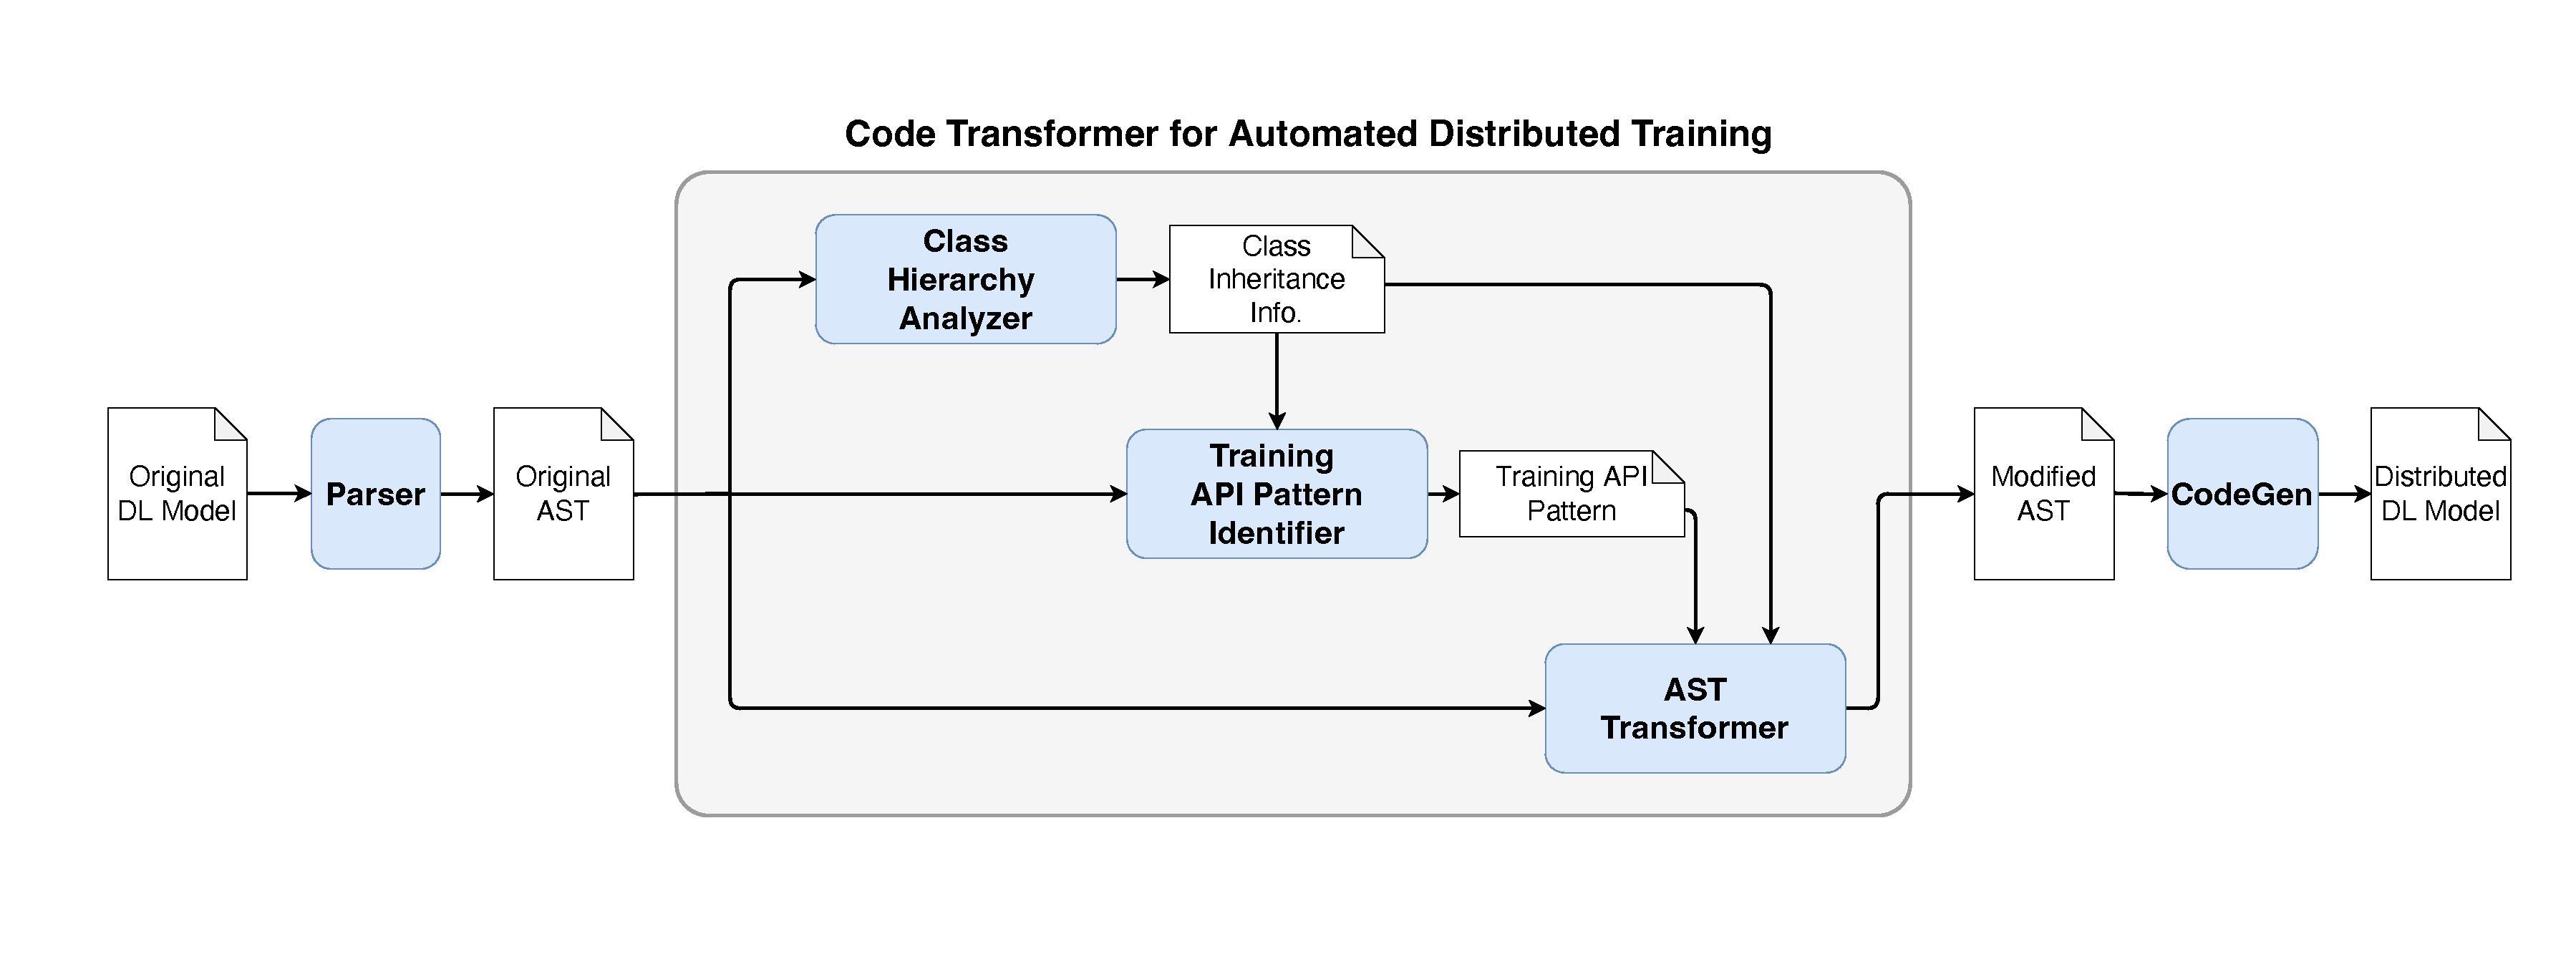
\includegraphics[width=\textwidth]{overview_diagram.pdf}
  \caption{Overall structure of the 
  automated transformation for distributed training}
  \label{sysarch}
\end{figure}

% main topic sentence for each paragraph

% 우리는 코드 변환을 기반을 기존의 모델을 자동으로 분산화하는 기법을 제안한다.
We propose the code transformation-based approach 
for automated distributed training of TensorFlow DL models.
As explained in the previous section, distributing TensorFlow DL models
with Horovod library requires adding and editing the original models.
Currently, the developers must fully understand the model codes and
manually rewrite them.
This also includes understanding the Horovod library usage by reading
the library documentation and code exmaples.
To ease the burden of the rewriting process, 
we utilize the code transformation technique to automatically rewrite the
input TensorFlow model code with Horovod library.

% 기존의 모델에 적용하는 코드 변환 규칙을 정의하기 위해 horovod 라이브러리 문서와
% 코드 예제를 검토했다. 그 결과로 TF 모델을 4가지로 분류하고 각 분류에 맞는
% 변환 규칙을 정의할 수 있었다.
To define the code transformation rule for distributed training of 
TensorFlow DL models,
we manually inspected the Horovod library documentation and code examples.
In this end, we identified four categories of TensorFlow DL models.
We define four \textit{training API patterns}, which are common code patterns of 
TensorFlow APIs appearing in each category of the TensorFlow DL models.
To categorize the TensorFlow DL models into one of the four patterns, 
we implemented the \textit{training API pattern identifier}. 
In this process, we identified that the training API pattern identifier 
must know the class inheritance relationship between TensorFlow library 
classes and user-defined classes.
To solve this problem, we also implemented the \textit{class hierarchy analyzer}
to retrieve the class inheritance information of the TensorFlow DL model.



% 우리 기법은 입력으로 주어진 TF 모델에서 먼저 API 패턴을 인식하고
% 해당 패턴에 맞는 코드 변환 규칙을 적용하는 방식으로 작동한다.
% 이를 위해 설계한 우리 기법의 overview는 피규어와 같다...
Figure \ref{sysarch} illustrates the overview of our approach.
Given the single-GPU model as an input, our approach parses the model codes
into ASTs in order to mechanically analyze and modify them.
We first analyze the class hierarchy of the input TensorFlow model
to produce the class inheritance information.
Then the training API pattern identifier uses the inheritance information to
identify the training API pattern of the input model.
Finally, the AST transformer selects the correct transformation rule
according to the training API pattern then apply the rule to the model ASTs.
The modified ASTs are finally converted into Python codes to return
the distriubted model as an output.

The following sections provide detailed explanation on the components of our
approach. The section \ref{sec:cha} describes the
necessity of class hierarchy analysis for our appraoch.
The section \ref{sec:pattern} describes the training API patterns and the
training API pattern identifier. The section \ref{sec:trans} describes the
formalization of the transformation rules for the training API patterns.
